\section{Estrutura da Rede Neural Artificial}

\begin{frame}{Sistema de Compressão}

\begin{figure}
    \centering
    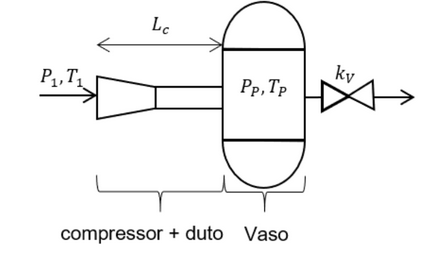
\includegraphics[width=0.6\linewidth]{figures/compressao.png}
    \caption{Sitema de Compressão retirado de Meira et al. (2021)}
    \label{fig:enter-label}
\end{figure}


\end{frame}
% Equações Governantes
\begin{frame}{Sistema de Compressão e Gás Natural}
    \begin{columns}[T] % [T] alinha as colunas pelo topo
        % Coluna da esquerda - Tabela
        \begin{column}{0.48\textwidth}
            \begin{block}{\centering Tabela de dados do sistema}
                \footnotesize
                \centering
                \begin{tabular}{ccc}
                    \toprule
                    \textbf{Variável} & \textbf{Valor} & \textbf{Unidade} \\
                    \midrule
                    $A_1$ & $2{,}6 \times 10^{-3}$ & m² \\
                    $v_P$ & $2{,}0$ & m³ \\
                    $L_C$ & $2{,}0$ & m \\
                    $k_v$ & $0{,}38$ & kg/(s·kPa) \\
                    $P_1$ & $4{,}5$ & MPa \\
                    $T_1$ & $300$ & K \\
                    $P_{\text{saída}}$ & $5{,}0$ & MPa \\
                    \bottomrule
                \end{tabular}
            \end{block}
        \end{column}

        % Coluna da direita - Composição e EoS
        \begin{column}{0.52\textwidth}
            \scriptsize
            O gás natural utilizado é rico em metano, com composição baseada em Chaczykowski (2009):
            
            \vspace{0.15cm}
            \begin{itemize}
                \item CH\textsubscript{4}: 98,34\% \quad C\textsubscript{2}H\textsubscript{6}: 0,61\%
                \item C\textsubscript{3}H\textsubscript{8}: 0,15\% \quad iC\textsubscript{4}H\textsubscript{10}: 0,03\%
                \item nC\textsubscript{4}H\textsubscript{10}: 0,03\% \quad CO\textsubscript{2}: 0,80\%
                \item Traços de: iC\textsubscript{5}H\textsubscript{12}, nC\textsubscript{5}H\textsubscript{12}, N\textsubscript{2}
            \end{itemize}

            \vspace{0.15cm}
            A equação de estado de Soave (1972) foi utilizada para modelar o comportamento termodinâmico do gás:

            \[
            P = \frac{R T}{V - b} - \frac{a(T)}{V(V + b)}
            \]

            com:
            \begin{itemize}
                \item \( a(T) \): fator de correção das forças intermoleculares
                \item \( b \): correção do volume molecular
            \end{itemize}
        \end{column}
    \end{columns}
\end{frame}



\begin{frame}{Equações Diferenciais do Sistema por Meira et al. (2021)}
    As equações diferenciais são dadas pelas seguintes expressões:
    \begin{align}
        \frac{d\dot{m}}{dt} &= \frac{A_1}{L_c}(P_2 - P_P) \tag{1} \\
        \frac{dV_P}{dt} &= -\frac{V_P^2}{v_{PM}} \left( \dot{m} - \alpha k_v \sqrt{P_P - P_{\text{out}}} \right) \tag{2} \\
        \frac{dT_P}{dt} &= \frac{V_P \dot{m}}{v_P M} \left( \frac{h_c - h_p}{C_V} \right)
        + \frac{R_a T_P}{C_V} \left[ T_P \left( \frac{\partial Z_P}{\partial T} \right)_{V_P} + Z_P \right]
        \frac{V_P}{v_P M} \left( \dot{m} - \alpha k_v \sqrt{P_P - P_{\text{out}}} \right) \tag{3}
    \end{align}

    \vspace{0.1cm}

    \begin{itemize}
        \item \( \dot{m} \): vazão mássica;
        \item \( V_P \), \( T_P \), \( Z_P \): volume molar, temperatura e fator de compressibilidade do gás no plenum;
        \item \( R_a \): constante dos gases ideais;
        \item \( M \): massa molar da mistura;
        \item \( h_1 \), \( h_p \), \( h_c \): entalpias na sucção, no vaso e na descarga, dependentes de \( T \), \( V \) e da composição;
        \item \( C_V \): capacidade calorífica a volume constante.
    \end{itemize}

\end{frame}

\begin{frame}{Variáveis Algébricas estimadas pelo Modelo Meira et al. (2021)}
    \scriptsize
    Além das equações diferenciais, o modelo estima 11 variáveis através das equações algébricas, correspondentes ao cálculo do mapa do compressor, da saída das condições do compressor e da equação de estado P(T,V)

    \vspace{0.3cm}

    \begin{multicols}{2}
    \begin{itemize}
        \item \( P_2 \): Pressão na saída do compressor
        \item \( T_2 \): Temperatura na saída do compressor
        \item \( V_2 \): Volume específico na saída do compressor
        \item \( T_{2s} \): Temperatura em um estado intermediário hipotético após a compressão isentrópica
        \item \( V_{2s} \): Volume específico em um estado intermediário hipotético após a compressão isentrópica
        \item \( P_P \): Pressão no Plenum
    \end{itemize}

    \columnbreak

    \begin{itemize}
        \item \( V_1 \): Volume específico na sucção
        \item \( V_{imp} \): Volume específico no impelidor do compressor
        \item \( T_{imp} \): Temperatura no impelidor do compressor
        \item \( V_{dif} \): Volume específico no difusor do compressor
        \item \( T_{dif} \): Temperatura no difusor do compressor
    \end{itemize}
    \end{multicols}

    \vspace{0.2cm}

    \end{frame}
\begin{frame}{Estrutura da Rede Neural Proposta}
    \vspace{-0.3cm}
    \begin{figure}
        \centering
        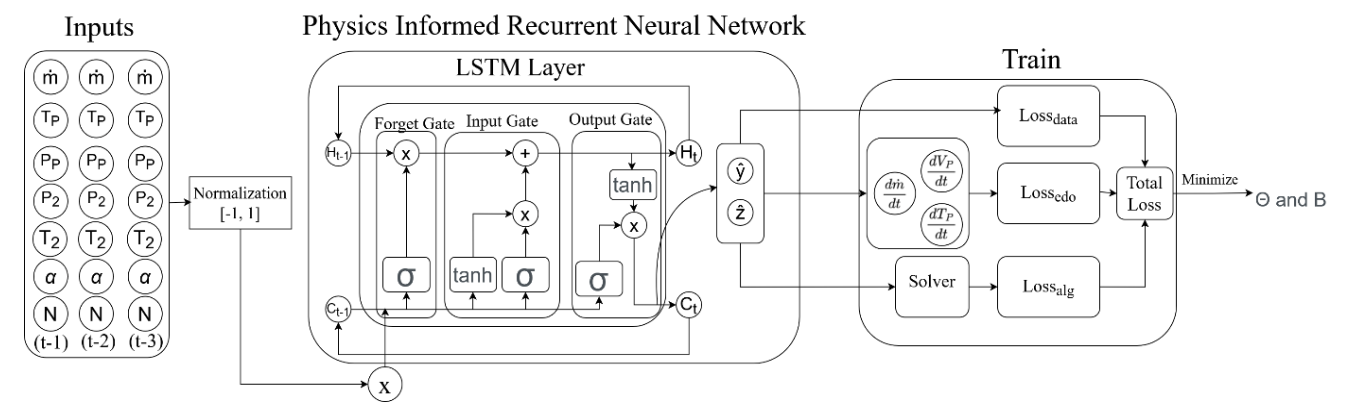
\includegraphics[width=1.0\textwidth]{figures/PIRNN.png} % Insira o caminho correto para a imagem
        \caption{\small Diagrama da arquitetura da PINN.}
    \end{figure}
\end{frame}
\begin{frame}{Função de Loss}
    \vspace{0.3cm}
    A equação geral da função de perda é:
    
    \[
    \text{Loss} = \frac{1}{N} \sum_{i=1}^{N} (\hat{y}_i^* - y_i^*)^2
    + \frac{1}{N} \sum_{i=1}^{N} \left( \frac{d\hat{y}_{i,\text{num}}}{dt} - \frac{d\hat{y}_{i,\text{an}}}{dt} \right)^2
    + \frac{1}{N} \sum_{i=1}^{N} (\hat{z}_i - z_i)^2
    \]

    \vspace{0.2cm}
    Onde:
        \begin{itemize}
        \item \( \hat{y} \): variáveis previstas pelas equações diferenciais (rede neural);
        \item \( \hat{y}^* \): variáveis previstas mensuráveis (saída da rede);
        \item \( \hat{z} \): variáveis algébricas previstas pela rede;
        \item \( z \): variáveis algébricas calculadas pelo solver externo.
     \end{itemize}
\end{frame}
\begin{frame}{Escolha dos Hiperparâmetros da rede}
    \vspace{0.3cm}
    \begin{itemize}
        \item \textbf{Número de camadas(LSTM):} 1
        \item \textbf{Taxa de aprendizado inicial (Learning Rate):} $1\cdot10^{-4}$
        \item \textbf{Tamanho da amostra por iteração(Mini batch):} 64
        \item \textbf{Número de neurônios na camada LSTM:} 128
        \item \textbf{Número de épocas durante o treinamento:} 200
        \item \textbf{Otimizador:} Adam
    \end{itemize}
\end{frame}